% Famous Experiments

\documentclass[11pt]{article}

\usepackage[a4paper, margin=1in]{geometry}

\usepackage{amsmath}

\usepackage{amssymb}

\usepackage[german]{babel}

\usepackage[autostyle=true]{csquotes}

\usepackage{libertine}

\usepackage[libertine]{newtxmath}

\usepackage{tikz}

\usepackage{gensymb}

\usepackage{fancyhdr}

\usepackage{amsfonts}

\usepackage{pgfplots}

\pgfplotsset{compat=1.10}

\usepackage{multicol}

\usepackage{caption}

\usepackage{floatrow}

\everymath{\displaystyle}

% Header / footer settings

\pagestyle{fancy}
\fancyhf{}
\renewcommand{\headrulewidth}{0.2mm}
\fancyhead[C]{Funktionen}
\renewcommand{\footrulewidth}{0.2mm}
\fancyfoot[L]{Peter Goldsborough}
\fancyfoot[C]{\thepage}
\fancyfoot[R]{\today}

\fancypagestyle{plain}{%
	\fancyhf{}
	\renewcommand{\headrulewidth}{0mm}%
	\renewcommand{\footrulewidth}{0.2mm}%
	\fancyfoot[L]{Peter Goldsborough}
	\fancyfoot[C]{\thepage}
	\fancyfoot[R]{\today}
}


\setlength{\headheight}{15pt}

\setlength{\parindent}{0pt}

\addtolength{\parskip}{\baselineskip}


\newcommand{\overbar}[1]{\mkern 1.5mu\overline{\mkern-1.5mu#1\mkern-1.5mu}\mkern 1.5mu}

\newcommand{\heading}[1]{\begin{center}\Huge \textbf{#1}\end{center}\par}

\newcommand{\sub}[1]{\vspace{\parskip}{\LARGE\textbf{#1}}}

\newcommand{\subsub}[1]{{\Large \textbf{#1}}}

\newcommand{\subsubsub}[1]{\textbf{#1}}

\newcommand{\colvec}[1]{\begin{pmatrix}#1\end{pmatrix}}

\newcommand{\extrapar}{\par\vspace{\baselineskip}}

\newcommand{\zitat}[1]{\foreignquote{german}{#1}}

\newcommand{\bolditem}[1]{\item \textbf{#1}}

\newcommand{\titleitem}[1]{\bolditem{#1}\par}

\newcommand{\defas}{ \dots \,\,}

\begin{document}
\thispagestyle{plain}

\heading{Famous Experiments}

\sub{Determination of the Wavelength of Light}

Through vacuum, all electromagnetic waves travel at the same speed: the speed of light. This speed is exactly $299 792 458\, m\, s^{-1}$ and is commonly rounded to $3 \cdot 10^8\, m\, s^{-1}$. There were two noteworthy attempts to determine this speed, the astronomical method of Ole Roemer from the year 1676 and the method of Armand Fizeau from the year 1849.

\subsub{The Astronomical Method of Roemer}

In the 17th century, the astronomer Ole Roemer was observing the eclipses of Io, one of Jupiter's moons. He noticed that when the earth was closest to Jupiter, the eclipse seemed to occur 11 minutes earlier than what estimates of the time predicted. Moreover, he noticed that when the earth had moved on in its orbital motion around the sun and was furthest from Jupiter, the eclipse of Io occured 11 minutes later than estimated. He therefore determined a time difference of 22 minutes for the eclipse of Io across the diameter of the earth's orbit around the sun. Dividing the displacement of the light between the closest and furthest distance between earth and Jupiter by the time taken resulted in the first historical estimate for the speed of light.

\begin{plot}
	% Sun at the center
	\draw [fill=yellow, yellow] (0, 0) circle [radius=0.35cm];

	% Orbit of the earth around the sun
	\draw (0, 0) circle [radius=1cm];

	% Earth, first position
	\draw [fill=cyan, cyan] (-1, 0) circle [radius=0.1cm];

	% Earth, second position
	\draw [fill=cyan, cyan] (1, 0) circle [radius=0.1cm];

	% Orbit of Jupiter around the sun
	\draw (0, 0) circle [radius=3cm];

	% Jupiter, first position
	\draw [fill=orange, orange] (-3, 0) circle [radius=0.2cm];

	% Jupiter, second position
	\draw [fill=orange, orange] 
		  (-2.6, {-sqrt(9 - 2.6^2)}) circle [radius=0.2cm];

	% First light
	\draw [->] (-2.8, 0) -- (-1.1, 0);

	% Second light
	\draw [->] (-2.4, {-sqrt(9 - 2.6^2)}) -- (0.9, 0);

	% Orbital diameter of earth
	\draw [<->] (-1, -1.5) -- (1, -1.5)
	      node [midway, below] {$3 \cdot 10^{11}\, m$};


	% Legend, sun
	\draw [fill=yellow, yellow] (4.5, 3)
	      circle [radius=0.35cm]
	      node [right, black] {\hspace{0.5cm} Sun};

	% Legend, jupiter
	\draw [fill=orange, orange] (4.5, 2)
	      circle [radius=0.2cm]
	      node [right, black] {\hspace{0.5cm} Jupiter};

	% Legend, earth
	\draw [fill=cyan, cyan] (4.5, 1)
	      circle [radius=0.1cm]
	      node [right, black] {\hspace{0.5cm} Earth};

\end{plot}

$$c = \frac{\Delta s}{\Delta t} = \frac{3 \cdot 10^11\, m}{22\, min \cdot 60\, s} = 2.3 \cdot 10^8\, m\, s^{-1}$$

\subsub{Method of Fizeau}

Another experiment to determine the speed of light was carried out by Armand Hippolyte Louis Fizeau in 1849. This time, the measurement was imprecise only by 2 percent compared to the actual value. His experimental setup, simply stated, included a light source (at the time a candle), a smaller semi-reflective mirror, a large mirror and a toothed wheel. The observer is behind the semi-reflective mirror, which was placed at an angle to the candle, such that the light hitting the mirror from the candle would reflect in the opposite direction of the observer. The large mirror was placed at a distance of 10 km from the rest of the setup. When the light reflected off the semi-reflective mirror would hit the large mirror, it would be reflected back to the observer and this time be let through by the semi-reflective mirror (this is the benefit of a \emph{semi-reflective} mirror). The toothed wheel, with a fixed number of $n$ teeth (notches) and a variable frequency was placed between the semi-reflective and far-away large mirror, at a small distance to the semi-reflective one. 

\begin{figure}[h!]
	\centering
	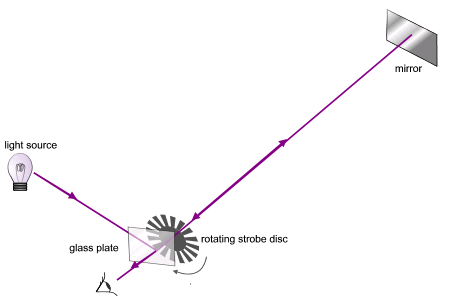
\includegraphics[scale=0.7]{img/fizeau}
	\caption{Fizeau's experimental setup}
\end{figure}

Armand Fizeau's reasoning was the following: given the right frequency of rotation, the light of the candle would pass through one tooth at one time and pass through the next with the full intensity. Knowing the frequency of rotation and the number of teeth in the wheel, he could then calculate the speed of light by dividing the pre-defined distance the light covered between the two teeth by the time it took for the wheel to move over from one tooth to the next. For this he defined three cases:

\begin{enumerate}
	\item The first case pertains to the situation in which the toothwheel is at rest. The light can pass through one tooth and is reflected through the same tooth. This yields the highest possible intensity of the light which serves as the reference intensity for the following cases.


	\item The second case occurs when the toothwheel is rotating at an imperfect frequency such that the light is blocked by a tooth in its path, either completely or partially. The intensity observed is lower than the reference intensity.

	\item The third case is the case in which the experiment is successful. The toothwheel is rotating at just the right frequency, meaning the light passes through one tooth, is reflected by the mirror at distance and passes through the \emph{next} tooth upon returning to the observer and the toothwheel.
\end{enumerate}

Given the determination of the right frequency for case three, the speed of light can be calculated. For this, the time must be determined during which one tooth moves on to the next. Given a frequency of rotation $f$ in Hertz, the period of one rotation can be calculated as the inverse of the frequency. This period must then be divided by the number of teeth $n$ to obtain the fraction of the period during which the wheel moves by exactly the distance of one tooth. The distance $s$ between the wheel and the mirror at distance is moreover multiplied by two, given that the path of the light includes the distance to and from the mirror. This yields the following expression for the speed of light given the parameters just described: $$c = \frac{\Delta s}{\Delta t} = \frac{2 \cdot s}{(f \cdot n)^{-1}} = 2 \cdot s \cdot f \cdot n$$

\end{document}